\documentclass[conference]{IEEEtran}
\usepackage{amsmath,amssymb}
\usepackage{graphicx}
\usepackage{booktabs,array,tabularx}
\usepackage{cite,url}
\usepackage{tikz}
\usetikzlibrary{positioning,arrows.meta}
\newcommand{\project}{Energy Detective}
\begin{document}
\title{Energy Detective: An Evidence-Traceable AI Agent for Household Electricity Analytics}
% Course draft: replace Group 20 with the confirmed English author names before a formal submission.
\author{\IEEEauthorblockN{Group 20}\IEEEauthorblockA{National Chung Hsing University\\Taichung, Taiwan}}
\maketitle

\begin{abstract}
Household electricity records can support energy management, yet interpreting time-series measurements and translating them into appropriate actions remains difficult for non-expert users. Natural-language energy assistants can simplify access to data, but inaccurate numerical claims, ambiguous time intervals, and unsupported causal explanations can undermine their usefulness. This paper proposes \project, a tool-based domain AI agent that supports electricity queries, period comparisons, anomaly candidate identification, next-hour forecasting, and evidence-informed recommendations. An agent coordinates controlled analytical tools, a versioned energy knowledge base, and an explicit evidence registry. A deterministic pre-response verification stage checks numerical values, timestamps, units, and evidence references, with at most one repair attempt. Evaluation is planned using the UCI Individual Household Electric Power Consumption dataset. Forecasts will be compared with persistence and daily seasonal-naive baselines using MAE and RMSE; an agent-level experiment will compare verified and unverified responses over 50 fixed tasks with three repetitions per condition. The expected contribution is a reproducible framework for assessing answer reliability and evidence traceability, rather than a claim of achieved energy savings. Experimental results are not yet available.
\end{abstract}
\begin{IEEEkeywords}
Domain AI agent, household electricity, evidence traceability, answer verification, load forecasting, energy analytics.
\end{IEEEkeywords}

\section{Introduction}
Residential energy management is an important part of energy efficiency. The International Energy Agency estimates that residential buildings account for approximately 70\% of building energy demand \cite{iea2025}. Providing households with timely information can influence consumption, as reported in field experiments on electricity feedback and behavioral interventions \cite{boomsma2025,paunov2026}. These studies motivate accessible analysis but do not establish that a conversational assistant will reduce electricity consumption.

A household member may ask which period consumed more electricity, whether unusually high consumption should be investigated, or how much electricity is likely to be consumed in the following hour. Reliable answers require more than natural-language fluency. Power measured in kilowatts (kW) must be integrated over time to calculate energy in kilowatt-hours (kWh); missing measurements must not be treated as zero. A rise in an appliance-group meter cannot establish which individual appliance caused it. Furthermore, predictions must be distinguished from historical measurements.

Recent energy-management agents combine language models with analysis and device-related tools \cite{he2025,jonah2026}. Their evaluation highlights the need to distinguish correct explanations, tool execution, and constraint satisfaction. Short-term forecasting studies similarly focus on predictive error rather than the evidential adequacy of conversational responses \cite{muqtadir2025}. A useful design question is therefore whether an explicit external verification and bounded repair mechanism can improve the reliability of household electricity analysis without excessive overhead.

\project{} addresses this question in a read-only historical replay setting with a cloud LLM planner, deterministic analytical tools, versioned domain knowledge, evidence recording, and a planned Streamlit interface. The contributions of this draft are:
\begin{itemize}
\item An architecture for five household electricity tasks with explicit measurement, data-availability, and inference constraints.
\item A structured evidence registry and bounded answer verification workflow for traceable numerical responses.
\item A chronological forecasting benchmark and a paired agent evaluation that measures reliability, coverage, appropriate limitations, and resource overhead.
\end{itemize}
These are design and evaluation contributions at the proposal stage. Neither a trained model nor completed agent experiments are claimed.

\section{Related Work}
\subsection{Household Energy Feedback}
Boomsma \textit{et al.} investigated real-time energy feedback in a randomized residential study \cite{boomsma2025}. Paunov \textit{et al.} compared social-comparison feedback with capability-building prompts in student housing \cite{paunov2026}. Their research motivates giving users understandable, actionable information while distinguishing answer quality from behavior change. Demand flexibility also distinguishes changing consumption timing from reducing total consumption \cite{ieaflex2025}; without tariffs or carbon-intensity data, the proposed agent will not quantify cost or emissions reductions.

\subsection{Energy Agents and Forecasting}
He and Jazizadeh proposed a context-aware LLM-based approach to human-centered energy management \cite{he2025}. Jonah \textit{et al.} considered tool-calling agents for household appliance scheduling \cite{jonah2026}. Such research supports tool-mediated interaction and highlights the importance of verifying constraints and results separately from explanatory text. The present work differs by targeting read-only historical analysis and explicit evidence consistency, not direct appliance control or scheduling.

Muqtadir \textit{et al.} examined ensemble models for next-hour residential load forecasting \cite{muqtadir2025}. B\'eraud \textit{et al.} considered interpretability in household energy estimation \cite{beraud2024}. Since datasets, horizons, and answer requirements differ, their numerical scores are not used as direct benchmarks for the proposed system. Table~\ref{tab:related} summarizes the research positioning.

\begin{table}[t]
\caption{Research positioning and proposed scope}
\label{tab:related}
\centering\footnotesize
\begin{tabularx}{\columnwidth}{@{}p{.23\columnwidth}X X@{}}
\toprule
Direction & Representative work & Scope of proposed evaluation \\
\midrule
Energy feedback & Field interventions \cite{boomsma2025,paunov2026} & Recommendation quality, not causal savings \\
Tool-based agents & Energy analysis and scheduling \cite{he2025,jonah2026} & Evidence-linked historical answers \\
Forecasting & Residential ensembles \cite{muqtadir2025,beraud2024} & Past-only hourly predictions vs. simple baselines \\
\bottomrule
\end{tabularx}
\end{table}

\section{System Design}
\subsection{Architecture and Task Scope}
Fig.~\ref{fig:architecture} shows the eight-module architecture. The LLM plans tool calls in a fixed historical context and interprets recorded results instead of performing unconstrained numerical calculations. A verifier checks draft claims before the interface presents the answer or limitations. The model ID will be fixed before experiments.

\begin{figure*}[t]
\centering
\resizebox{\textwidth}{!}{%
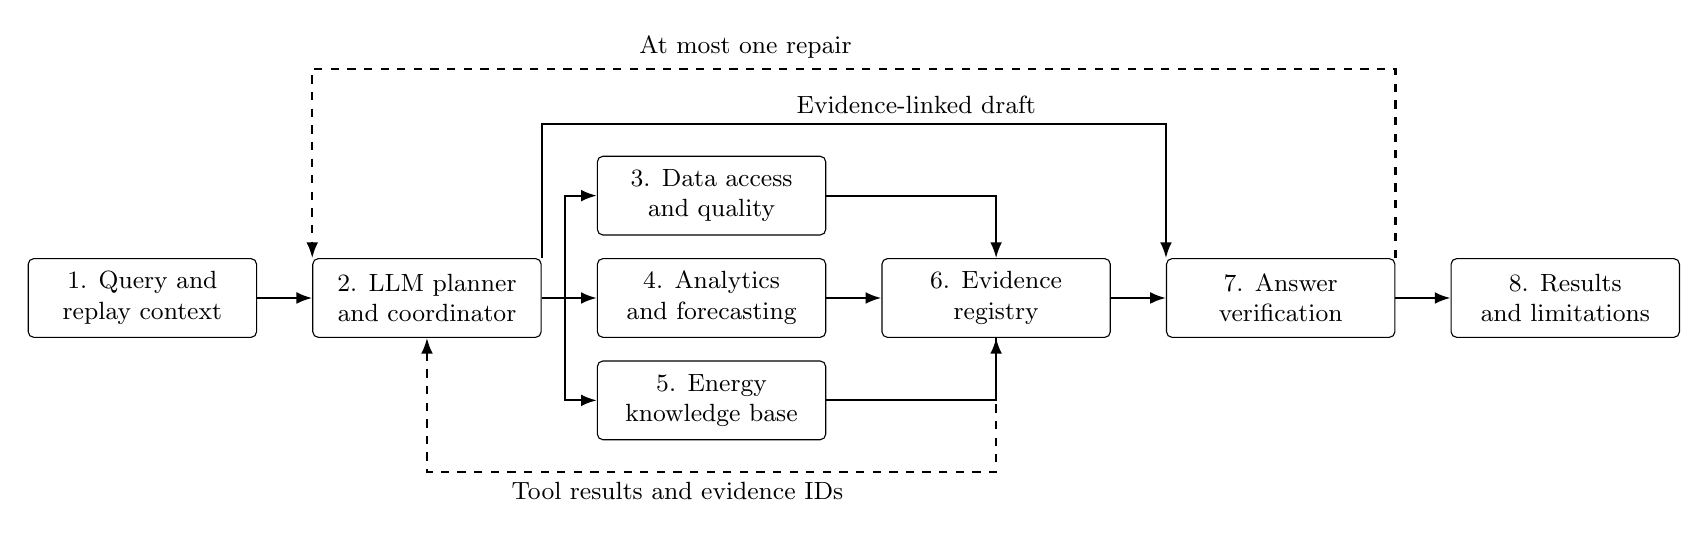
\begin{tikzpicture}[font=\small,box/.style={draw,rounded corners=2pt,align=center,minimum height=10mm,minimum width=29mm,inner sep=4pt},line/.style={-{Latex[length=2mm]},thick},node distance=7mm and 7mm]
\node[box] (input) {1. Query and\\replay context};
\node[box,right=of input] (agent) {2. LLM planner\\and coordinator};
\node[box,right=of agent,yshift=13mm] (data) {3. Data access\\and quality};
\node[box,right=of agent] (analytics) {4. Analytics\\and forecasting};
\node[box,right=of agent,yshift=-13mm] (knowledge) {5. Energy\\knowledge base};
\node[box,right=of analytics] (evidence) {6. Evidence\\registry};
\node[box,right=of evidence] (check) {7. Answer\\verification};
\node[box,right=of check] (output) {8. Results\\and limitations};
\draw[line] (input)--(agent);
\draw[line] (agent.east) -- ++(3mm,0) |- (data.west);
\draw[line] (agent)--(analytics);
\draw[line] (agent.east) -- ++(3mm,0) |- (knowledge.west);
\draw[line] (data.east) -| (evidence.north);
\draw[line] (analytics)--(evidence);
\draw[line] (knowledge.east) -| (evidence.south);
\draw[line] (evidence)--(check);
\draw[line] (check)--(output);
\draw[line] (agent.north east) -- ++(0,17mm) -| node[pos=.30,above]{Evidence-linked draft} (check.north west);
\draw[line,dashed] (check.north east) -- ++(0,24mm) -| node[pos=.30,above]{At most one repair} (agent.north west);
\draw[line,dashed] (evidence.south) -- ++(0,-17mm) -| node[pos=.28,below]{Tool results and evidence IDs} (agent.south);
\end{tikzpicture}}
\caption{Proposed architecture. Analytical tools receive a fixed read-only context; the shared evidence registry supports both the planner and external response checks. Dashed paths indicate feedback rather than new evidence sources.}
\label{fig:architecture}
\end{figure*}

\begin{table}[t]
\caption{Supported tasks and intended output}
\label{tab:tasks}
\centering\footnotesize
\begin{tabularx}{\columnwidth}{@{}p{.24\columnwidth}X@{}}
\toprule
Task & Output and interpretation \\
\midrule
Query & Energy (kWh), interval, and coverage \\
Comparison & Absolute difference; percentage only with a valid nonzero reference \\
Anomaly & Candidate flag and historical reference statistics, not a fault diagnosis \\
Forecast & Labeled estimate for the next hour; model and cutoff \\
Advice & Evidence-supported checks, conditions, and limits \\
\bottomrule
\end{tabularx}
\end{table}

Table~\ref{tab:tasks} summarizes the five tasks. Ambiguous requests trigger clarification; insufficient data, evidence, or service availability triggers explicit limitations rather than invented answers.

\subsection{Dataset and Historical Replay}
The UCI Individual Household Electric Power Consumption dataset contains approximately 2.08 million one-minute observations from a single home in France, recorded from December 2006 to November 2010 \cite{uci2006}. Its measurements include whole-home active power and three group-level sub-metering values. Some measurements are missing. The dataset is historical, not representative of all homes, and does not identify individual appliance causes or confirmed energy waste.

Let $h$ be the fixed replay boundary on the dataset's recorded clock, $I=[a,b)$ be a requested time interval, and $V_I$ be its set of valid, nonconflicting minute measurements. For historical analyses, $b\le h$ and only timestamps strictly earlier than $h$ are visible. For valid minute-average active power $P_i$ in kW and sub-metered energy $e_i$ in Wh,
\begin{align}
E_{\mathrm{whole}}(I)&=\sum_{i\in V_I}P_i/60,\label{eq:whole}\\
E_{\mathrm{sub}}(I)&=\sum_{i\in V_I}e_i/1000.\label{eq:sub}
\end{align}
Both sums are in kWh. Coverage is $c(I)=|V_I|/|G_I|$, where $G_I$ is the set of expected minute positions in the interval. A complete hour contains 60 distinct valid measurements; conflicting duplicates invalidate the affected minute. An incomplete interval returns only an observed partial energy and its coverage. An empty interval of valid readings yields a limitation, not a zero-consumption claim. A full-day comparison requires both full-day totals, and relative change is undefined if the reference energy equals zero.

\subsection{Anomaly Candidate Identification}
For a complete target hour beginning at $s$, construct a reference set $B_s$ from complete historical hours ending no later than $s$, within the preceding 56 days, with matching hour of day and weekday/weekend type. Let $m_s=\mathrm{median}(B_s)$ and $d_s=\mathrm{median}(|B_s-m_s|)$ be its median and median absolute deviation. The modified score \cite{nistoutlier} is
\begin{equation}
 z_s=\frac{0.6745(x_s-m_s)}{d_s}.
\end{equation}
The initial design flags $|z_s|>3.5$ only when there are at least 14 reference values and $d_s>0$. Otherwise, it reports the specific limitation or an observable difference. This is a candidate detection heuristic, not a calibrated failure probability or proof of energy waste; a reference sample cannot include the target hour itself.

\subsection{Next-Hour Forecasting}
The target $y_h$ is the complete electricity consumption for $[h,h+1\mathrm{h})$. The feature vector comprises hourly energy at lags 1, 2, 24, and 168, past 3- and 24-hour means and standard deviations, and calendar features known at $h$. A Random Forest regressor is the initial candidate with 200 trees, maximum depth 12, minimum leaf size 5, and random seed 42. No data at or after $h$ may appear in its features. Training artifacts must have a cutoff no later than the query replay boundary. Missing required values or an unavailable model cause a labeled limitation rather than an invented forecast.

Persistence predicts $\hat y_h=y_{h-1}$; daily seasonal-naive predicts $\hat y_h=y_{h-24}$. If a candidate model is unavailable, valid baselines may be returned with their method names, but never presented as Random Forest results. A point forecast is not a guarantee or an observed result.

\section{Evidence and Response Verification}
\subsection{Domain Knowledge and Evidence Contract}
A small, curated knowledge base will contain ten source-linked rules covering power and energy, metering granularity, missing data, comparable intervals, zero reference values, anomaly interpretation, prediction uncertainty, differing energy-management goals, behavior change, and generalization. Keyword/concept retrieval is sufficient for the initial design. Knowledge entries support interpretations but cannot substitute for the actual data needed for a specific causal claim.

Each tool invocation produces a structured evidence record: result identifier, replay boundary, source or dataset version, interval and field, tool/model version, arguments, data coverage and quality status, result values with units, and success or failure status. Charts and textual claims refer to the same record IDs. A structured draft binds each verifiable claim to an existing evidence identifier. No citations are invented for missing records.

\subsection{Bounded Agent Workflow}
The planner selects a clarification, a tool invocation, or a draft. The following procedure is the proposed control loop; $c$ counts attempted agent-initiated calls, including failures, and $r$ counts repairs. Internal tool checks do not consume additional agent calls.
\begin{figure}[t]
\centering\footnotesize
\begin{tabularx}{\columnwidth}{@{}rX@{}}
\toprule
\multicolumn{2}{@{}l}{\textbf{Algorithm 1: Evidence-linked agent loop}}\\
\midrule
1 & Freeze replay context; initialize registry $E$, $c=0$, $r=0$.\\
2 & Request next planner action using context and $E$.\\
3 & If clarification: return a clarification and end task.\\
4 & If tool: if $c=8$, return verified evidence or limitation.\\
5 & Otherwise increment $c$; execute guarded tool; log result or failure; go to line 2.\\
6 & If invalid action or service error: return limitation.\\
7 & Bind draft claims to $E$; verify values, units, intervals, directions, references, and required limitations.\\
8 & If checks pass: present answer, evidence, and limits.\\
9 & If checks fail and $r=0$: set $r=1$, pass failed checks to planner; go to line 2.\\
10 & Otherwise return only verified evidence or an explicit limitation.\\
\bottomrule
\end{tabularx}
\caption{Proposed bounded response verification and repair loop.}
\label{fig:algorithm}
\end{figure}
The workflow in Fig.~\ref{fig:algorithm} never resets the eight-call budget during repair. Deterministic checks can compare a rounded claim to its evidence within the appropriate rounding tolerance, e.g., 0.005 when two decimal places are displayed, plus negligible floating-point tolerance. Numeric checks cannot establish the validity of every free-text explanation; human assessment remains necessary for causal language and advice. When verification fails after one repair, a fixed response exposes only confirmed evidence or the reason no supported answer is available.

\section{Evaluation Plan}
\subsection{Research Questions}
RQ1: Can past-only Random Forest forecasting outperform persistence and daily seasonal-naive baselines? RQ2: How correctly can the agent complete the five task types, particularly for dates, units, and numeric results? RQ3: Does external verification and bounded repair improve evidence consistency and appropriate limitation handling, and what overhead does it introduce?

\subsection{Forecasting Experiment}
The hourly grid will be split chronologically into 70\% training, 15\% validation, and 15\% test. The initial parameters may be refined using training and validation only. After settings are frozen, models may be refitted on the first 85\% before a final test evaluation; future test targets are excluded from tuning. Models and simple baselines will be compared at common eligible forecast origins with valid targets, while reporting each method's availability and sample counts separately. For predictions $\hat y_i$ and measurements $y_i$ at $n$ common origins,
\begin{align}
\mathrm{MAE}&=\frac{1}{n}\sum_{i=1}^n|y_i-\hat y_i|,\\
\mathrm{RMSE}&=\sqrt{\frac{1}{n}\sum_{i=1}^n(y_i-\hat y_i)^2}.
\end{align}
Anomaly handling will be tested against deterministic rule expectations and boundary cases, not labeled fault-detection accuracy because the dataset lacks confirmed anomaly causes.

\subsection{Agent-Level Paired Comparison}
An independent 10-task pilot will refine tool descriptions and task format. The formal benchmark will contain 50 fixed questions: ten per task type, with six ordinary and four boundary cases per type. Boundary cases include missing measurements, ambiguous dates, zero reference values, insufficient anomaly baselines, unavailable models, and tool failures. Each question fixes replay time, visible data view, reference answer or limitation expectation, and grading rubric. Formal forecast replay times are selected from the final test interval, with training cutoff checked. Masked-data experiments use separate read-only views, preserving original data.

Two conditions use the same frozen model, dataset, tools, knowledge, evidence logging, answer format, initial instructions, and maximum eight tool attempts. Condition A disables external verification and repair; condition B enables both. Each condition performs three repetitions per question, producing $50\times2\times3=300$ planned task executions, not 300 API calls. Individual failures are retained. Repeated runs on the same question are not treated as independent questions; per-question paired summaries and per-task-category results will be reported.

\begin{table}[t]
\caption{Planned agent evaluation metrics}
\label{tab:metrics}
\centering\footnotesize
\begin{tabularx}{\columnwidth}{@{}p{.30\columnwidth}X@{}}
\toprule
Metric & Operational criterion \\
\midrule
Task completion & Satisfies reference answer or correct limitation \\
Numeric correctness & Required value, date, unit, and direction fields match \\
Evidence consistency & Verifiable claims supported by recorded results; report coverage alongside \\
Boundary handling & Appropriate limitation/clarification; ordinary-task unnecessary refusals reported separately \\
Recommendation quality & Two reviewers score support, inference limits, and actionability, each 0--2 \\
Overhead & Latency, tool attempts, repairs, model usage, and available cost \\
\bottomrule
\end{tabularx}
\end{table}
The metrics in Table~\ref{tab:metrics} separate answer completion from consistency so the system cannot appear more reliable merely by omitting difficult claims. Missing required fields count as failures. Two team reviewers independently assess recommendations and boundary reasoning, report initial agreement, and document disagreements. The comparison estimates the combined verification-and-repair effect. Model, data, tool, task, and generation versions will be frozen before testing.

\section{Expected Outcomes and Limitations}
The expected outputs are an implementation-ready specification, evidence-linked answers, and reproducible evaluation records. We hypothesize that verification reduces inconsistent responses at the cost of latency or model usage. No measured improvement or energy savings is reported.

Several limitations remain. The single historical household does not represent modern Taiwanese homes, multiple household types, or appliance-level behavior. Missing data may reduce forecast coverage. The dataset lacks confirmed causes of abnormal consumption, tariff and emissions context, and post-advice behavior. Rule-based verification cannot guarantee semantic correctness, and model version changes may affect reproducibility. Future work should test additional homes, evaluate sensitivity to missing data and thresholds, and separately study actual household adoption and energy outcomes. This design does not control physical appliances.

\section{Conclusion}
This paper proposes \project, a household electricity analytics agent that combines controlled analysis, source-linked domain knowledge, and evidence-aware response verification. Its key design choice is the separation of numerical computation from language generation with fixed historical visibility and bounded repair. A planned chronological forecast benchmark and paired agent experiment will establish the accuracy, limitations, and overhead of the proposed approach. Implementation and empirical validation remain future work.

\begin{thebibliography}{00}
\bibitem{iea2025} International Energy Agency, \emph{Energy Efficiency 2025}, Nov. 2025. [Online]. Available: \url{https://www.iea.org/reports/energy-efficiency-2025}
\bibitem{boomsma2025} M. Boomsma, K. Vringer, and D. van Soest, ``The impact of real-time energy consumption feedback on residential gas and electricity usage,'' \emph{Journal of Environmental Economics and Management}, vol. 132, Art. no. 103163, 2025, doi: 10.1016/j.jeem.2025.103163.
\bibitem{paunov2026} Y. Paunov, T. Gr\"une-Yanoff, C. Marchionni, and C. Schwirplies, ``A randomized field experiment comparing nudges and boosts for household electricity conservation in student housing,'' \emph{Scientific Reports}, vol. 16, Art. no. 27689, 2026, doi: 10.1038/s41598-026-69386-6.
\bibitem{he2025} T. He and F. Jazizadeh, ``Context-aware LLM-based AI agents for human-centered energy management systems in smart buildings,'' arXiv:2512.25055v1, 2025.
\bibitem{jonah2026} S. Jonah, Q. Moses, A. Babatunde, M. Ajao-Olarinoye, and D. Bammeke, ``LLMs for agentic home energy management,'' arXiv:2607.04569v2, 2026.
\bibitem{muqtadir2025} A. Muqtadir, B. Li, Z. Ying, C. Songsong, and S. N. Kazmi, ``Nowcasting the next hour of residential load using boosting ensemble machines,'' \emph{Scientific Reports}, vol. 15, Art. no. 7157, 2025, doi: 10.1038/s41598-025-91767-6.
\bibitem{ieaflex2025} International Energy Agency, \emph{The Value of Demand Flexibility: Benefits beyond Balancing}, Dec. 2025. [Online]. Available: \url{https://www.iea.org/reports/the-value-of-demand-flexibility}
\bibitem{beraud2024} P. B\'eraud \textit{et al.}, ``An explainable machine learning approach for energy forecasting at the household level,'' arXiv:2410.14416v1, 2024.
\bibitem{uci2006} G. Hebrail and A. Berard, ``Individual Household Electric Power Consumption,'' UCI Machine Learning Repository, dataset, 2006, doi: 10.24432/C58K54.
\bibitem{nistoutlier} NIST/SEMATECH, ``Detection of outliers,'' \emph{e-Handbook of Statistical Methods}, Sec. 1.3.5.17. [Online]. Available: \url{https://www.itl.nist.gov/div898/handbook/eda/section3/eda35h.htm}
\end{thebibliography}

\end{document}
